\documentclass[10pt,a4paper]{article}
\usepackage[latin1]{inputenc}
\usepackage{amsmath}
\usepackage{amsfonts}
\usepackage{amssymb}
\usepackage{graphics} 
\usepackage{graphicx}
\usepackage{float}
\usepackage{subfigure}

\author{Ana Huaman}
\title{ \vspace{-10ex}Homework 1 - RRR Arm}
\begin{document}
\maketitle

\section{Question}
The figure shows a RRR arm picking up containers filled with fluid from a lower conveyer belt and moving them to an upper conveyor bel. To avoid spilling, the containers must remain vertical. The robot end-effector moves on a series of straight line paths at 1 unit/sec to make the transfers. The length of the moving links are 3, 4 and 1 units and the coordinate origin is at the first joint. The conveyor dimensions are 2 by 1/2 units and the thickness of the sides and bottom are negligible.

\subsection{ Reverse displacement analysis}
Design a piecewise continuous trajectory for the robot. Ensure you pick enough data points to have a relatively smooth trajectory. There must be no interference of the robot or container with either conveyor. Plot the joint angles vs time on three separate plots. Be sure to use the same angle conventions as in the notes. This data could be used to control the joint motors. Hand in the joint plots.

\subsubsection*{Solution}
Considering:
\begin{itemize}
\item{ $q_{1}:$ Joint 1 angle }
\item{ $q_{2}:$ Joint 2 angle }
\item{ $q_{3}:$ Joint 3 angle }
\item{ $O_{x}, O_{y}:$ Location of joint 1 (fixed) }
\item{ $e_{x}, e_{y}$: Location of the end effector point}
\end{itemize}

The inverse analysis, considering that the third link is always vertical is:
\[ \begin{matrix}
 q_{2} = cos^{-1} \left(  \dfrac{ L_{1}^{2} + L_{2}^{2} - h^{2}}{2L_{1}L_{2}} \right) - \pi  \\
q_{1} = cos^{-1} \left(  \dfrac{ L_{1}^{2} + h^{2} - L^{2}}{2L_{1}h} \right) + \tan^{-1} \left( \dfrac{L_{3} + e_{y} - O_{y}}{e_{x} - O_{x}}\right)  \\
q_{3} = -\dfrac{\pi}{2} - q_{1} - q_{2} 
\end{matrix} \]

where:

\[ h = \sqrt{ (e_{x} - O_{x})^{2} + (L_{3} + e_{y} - O_{y})^{2} }\]

Given $(e_{x},e_{y})$ we can calculate the joint values. For the plots below we used the following \textit{end effector} via points:

\[ (8.5, 1.0),(8.5,2.0),(6.5,2.0),(6.5,6.0),(8.5,6.0),(8.5,5.0) \]

and interpolate between them with a step size of 0.02 units (executed in 0.02 seconds according to the rate of 1 unit/sec). The resulting plots are shown below:

	\begin{figure}[H]
	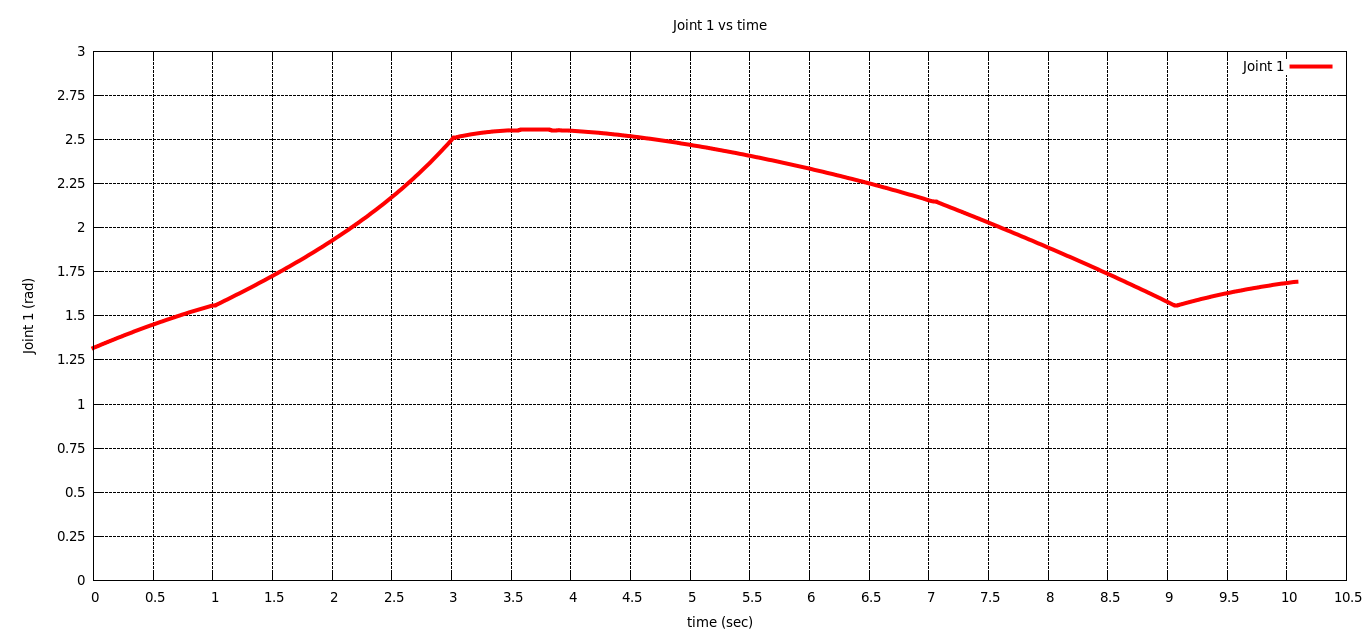
\includegraphics[angle = 0, scale = 0.3]{figures/Joint1.png} 
	\label{fig:Joint1}
	\caption{ Joint 1(rad) vs time(seconds)}
	\end{figure}

	\begin{figure}[H]
	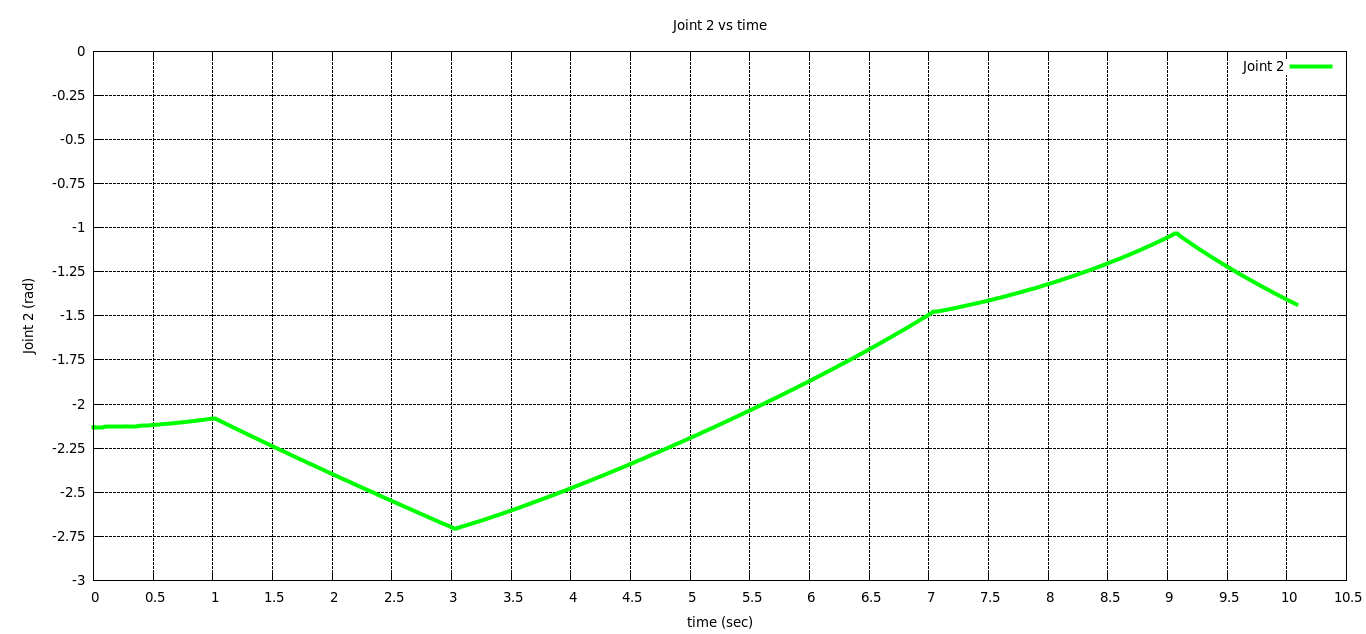
\includegraphics[angle = 0, scale = 0.3]{figures/Joint2.png} 
	\label{fig:Joint2}
	\caption{ Joint 2(rad) vs time(seconds)}
	\end{figure}
	
    \begin{figure}[H]
	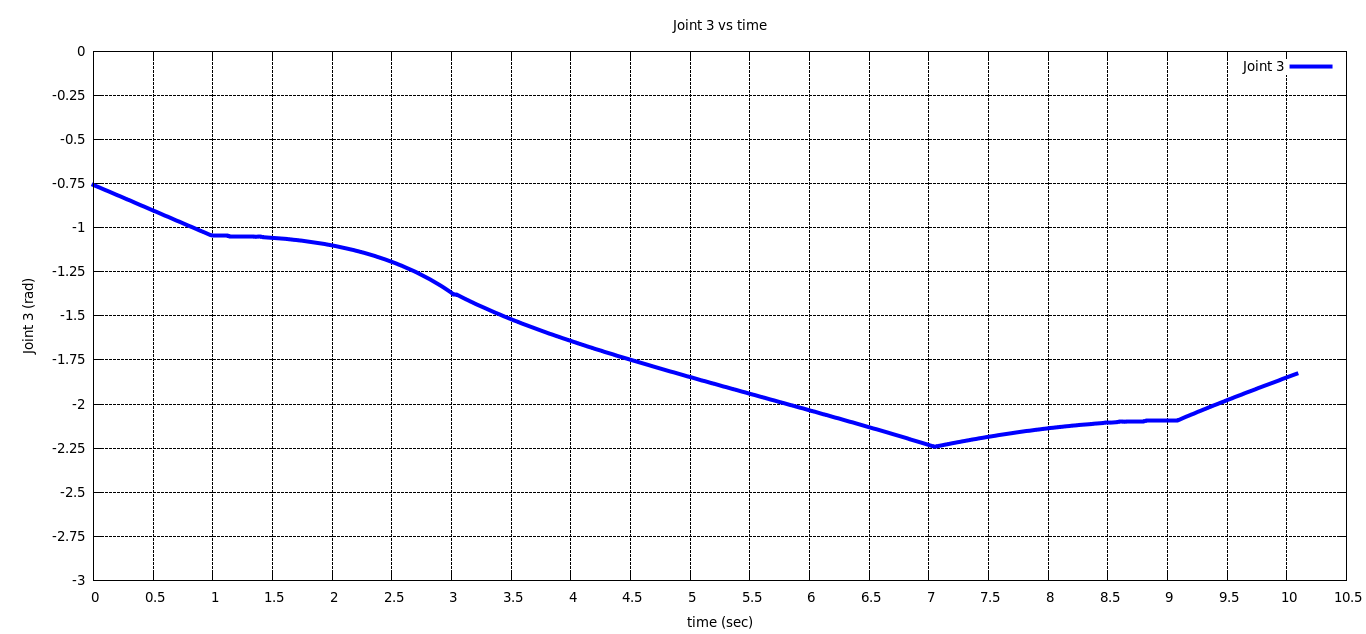
\includegraphics[angle = 0, scale = 0.3]{figures/Joint3.png} 
	\label{fig:Joint3}
	\caption{ Joint 3(rad) vs time(seconds)}
	\end{figure}

\subsection{ Forward displacement analysis} 
Use the joint angles to determine the locations of joints 2 and 3 and point e along the paths. Draw the robot links as a series of straight lines to simulate it moving on the path. (Feel free to embellish the drawing, like adding joints, etc. though it is not necessary). Hand in plots of the
robot along the path.

\subsubsection*{Plots}
The forward kinemtatics is pretty direct. The formulas used are:

\[ \begin{matrix}
P_{x}(q_{2}) = O_{x} + L_{1} \cos(q_{1}) \\
P_{y}(q_{2}) = O_{y} + L_{1} \sin(q_{1}) \\
P_{x}(q_{3}) = P_{x}(q_{2}) + L_{2} ( \cos(q_{1} + q_{2}) ) \\
P_{y}(q_{3}) = P_{y}(q_{2}) + L_{2} ( \sin(q_{1} + q_{2}) ) \\
P_{x}(e) = P_{x}(q_{3}) \\
P_{y}(e) = P_{y}(q_{3}) - L_{3}
\end{matrix} \]

Shown below for each indicated point ($P(q_{2})$, $P(q_{3})$ and $P(e)$). Note that for $P(q_{2})$, since it is attached to the fixed joint 1, the displacement pretty much reflects a circle arc.

Also note that the displacement of $P(q_{3})$ and $P(e)$ are only different in one unit (or $L_{3}$ ) along Y axis, which is understandable since the link $L_{3}$ remains vertical through the whole trajectory

	\begin{figure}[H]
	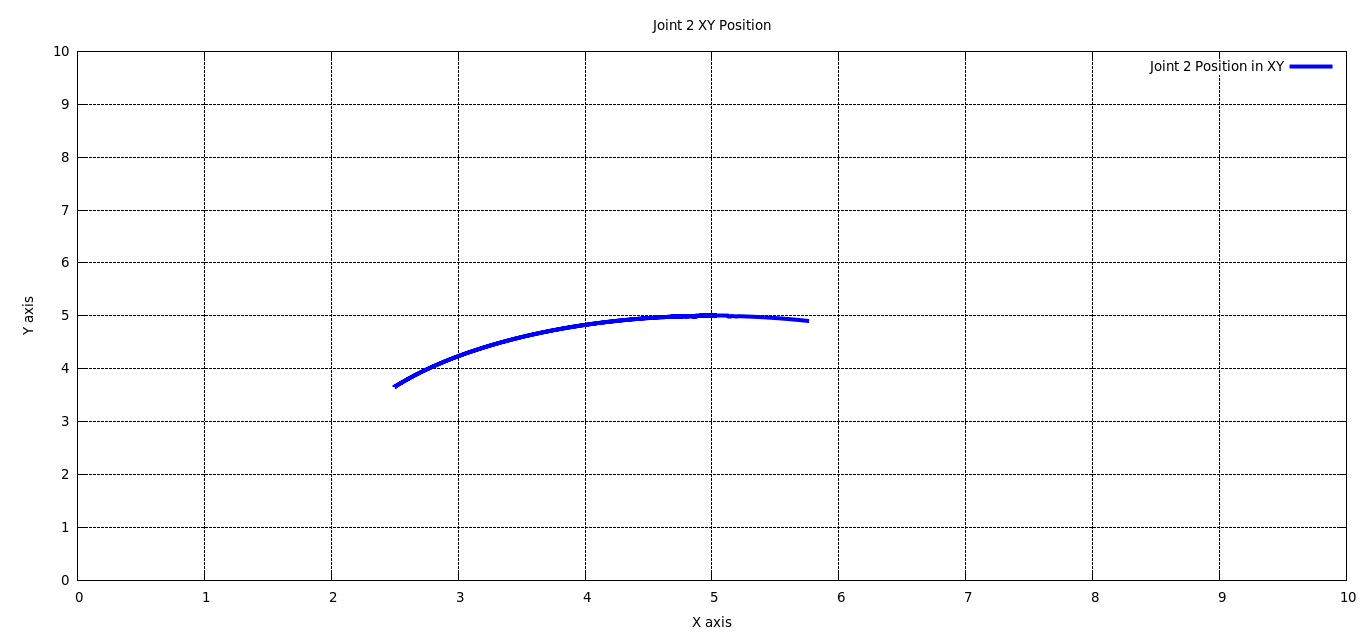
\includegraphics[angle = 0, scale = 0.3]{figures/Q1Joint2Pos.png} 
	\label{fig:Q1Joint2Pos}
	\caption{ Joint 2 - XY Position}
	\end{figure}

	\begin{figure}[H]
	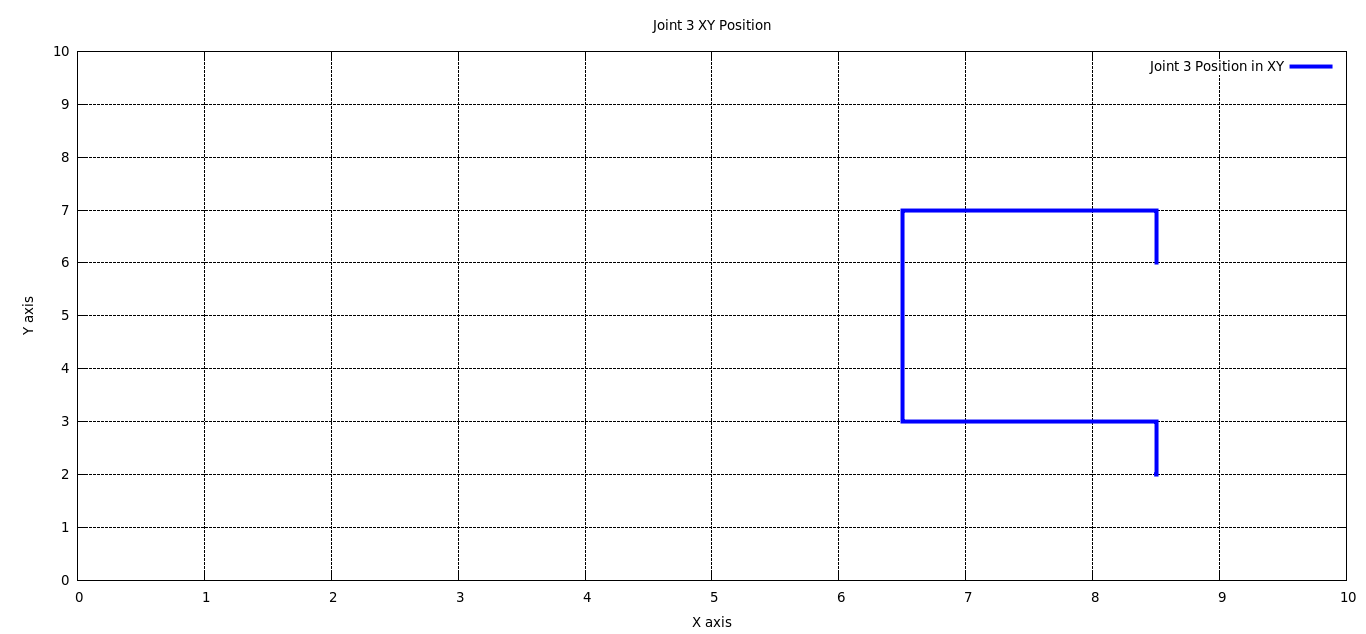
\includegraphics[angle = 0, scale = 0.3]{figures/Q1Joint3Pos.png} 
	\label{fig:Q1Joint3Pos}
	\caption{ Joint 3 - XY Position}
	\end{figure}
	
    \begin{figure}[H]
	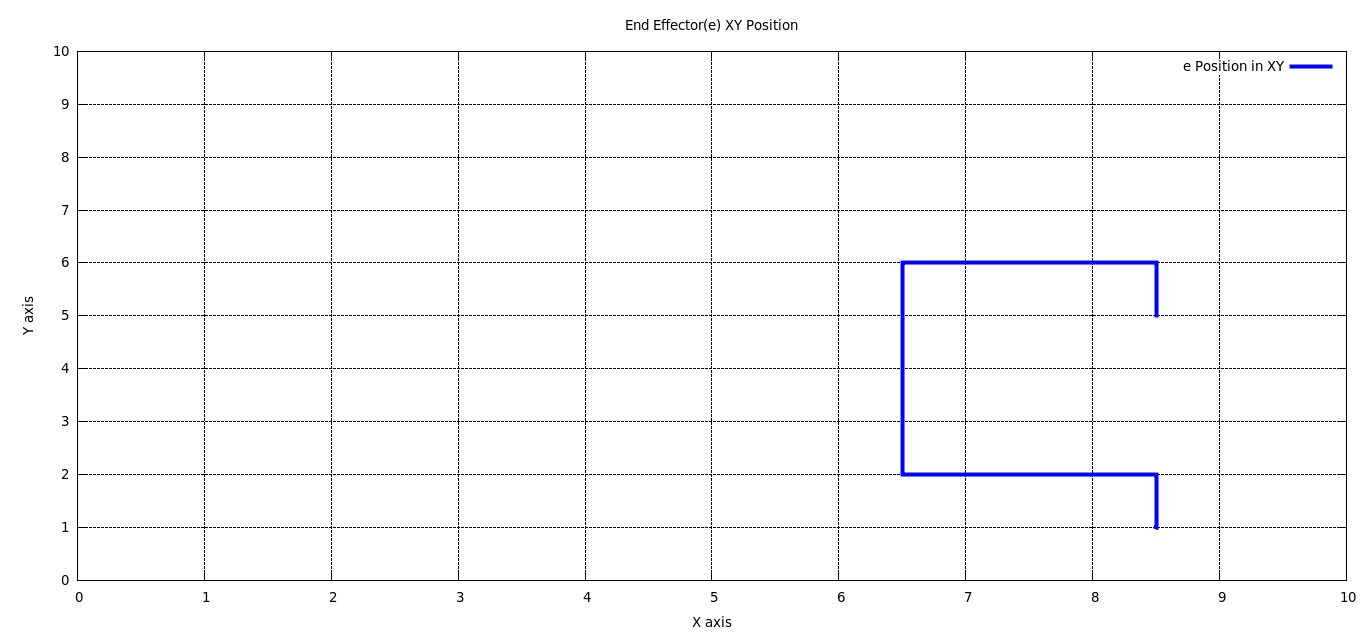
\includegraphics[angle = 0, scale = 0.3]{figures/Q1EEPos.png} 
	\label{fig:Q1EEPos}
	\caption{ End Effector e - XY Position}
	\end{figure}


And here some robot plots. There is a video attached to this assignment with the complete trajectory:

	\begin{figure}[h]
			\centering
			  \subfigure[Position 0]{
			  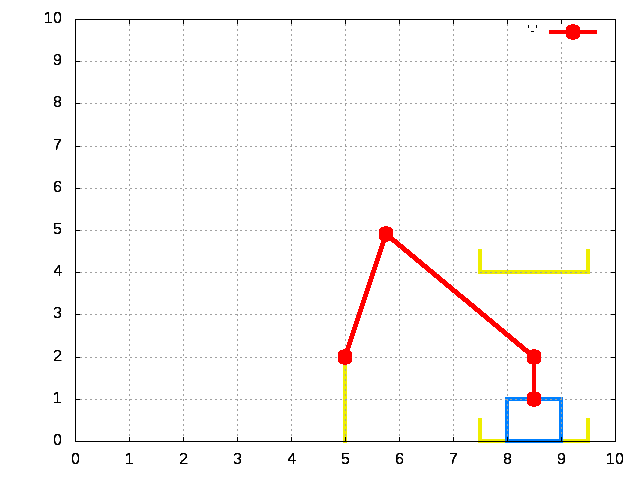
\includegraphics[scale=0.25]{figures/Q2Pos0.png} 
	          \label{fig:Q2Pos0}
              }
              \subfigure[Position 1]{
	          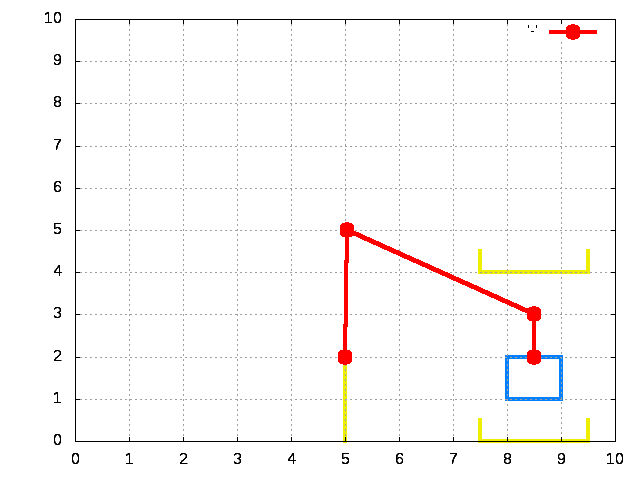
\includegraphics[scale=0.25]{figures/Q2Pos1.png} 	
	          \label{fig:Q2Pos1}
              }\\
			  \subfigure[Position 2]{
			  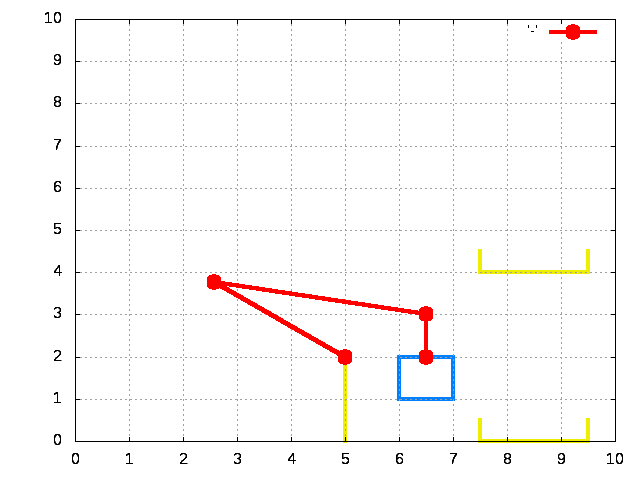
\includegraphics[scale=0.25]{figures/Q2Pos2.png} 
	          \label{fig:Q2Pos2}
              }
              \subfigure[Position 3]{
	          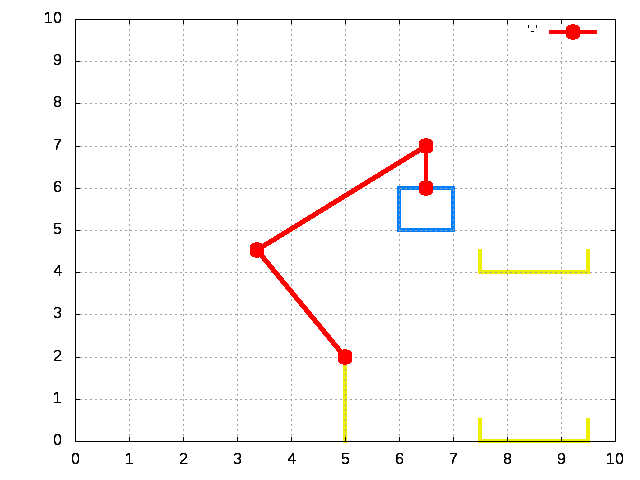
\includegraphics[scale=0.25]{figures/Q2Pos3.png} 	
	          \label{fig:Q2Pos3}
              }\\
              \subfigure[Position 4]{
			  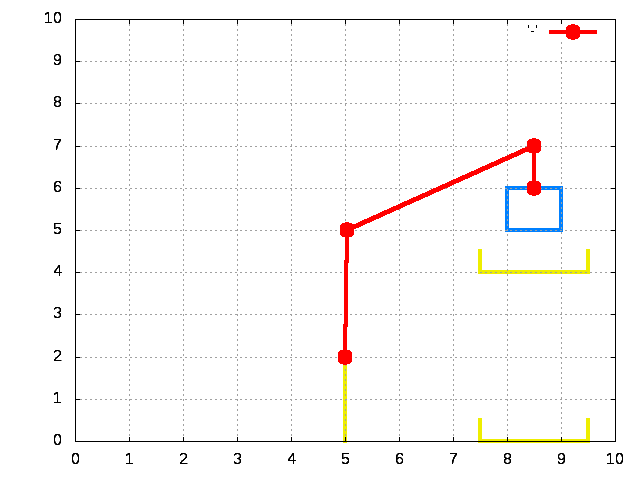
\includegraphics[scale=0.25]{figures/Q2Pos4.png} 
	          \label{fig:Q2Pos4}
              }
              \subfigure[Position 5]{
	          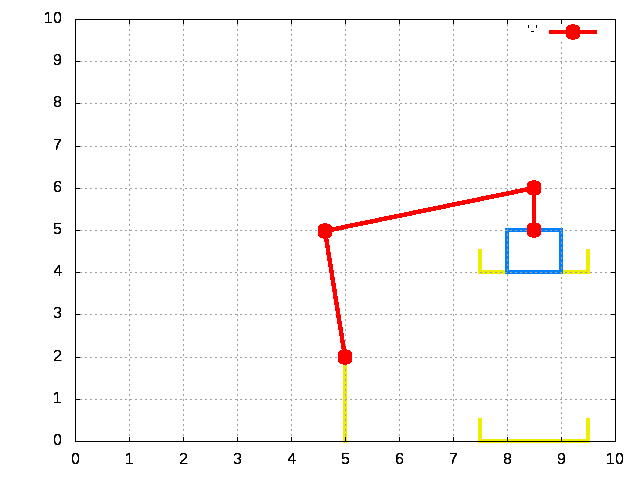
\includegraphics[scale=0.25]{figures/Q2Pos5.png} 	
	          \label{fig:Q2Pos5}
              }              
            \caption{ Robot poses for the trajectories plotted for question 2 }
            \label{fig:Q2}
	\end{figure}


\subsection{ Joint control} 
The robot controller has died and it must be controlled manually using a button box which can only control one joint at a time and you want to minimize the number of moves to save time. Also the containers are empty so the orientation along the path is not important. Solve the problem any way you can. Hand in plots of the robot along the path. (Hint: begin at the goal and work backwards to the start.)

\subsubsection*{Plots}
From observing question 1 and 2, we may say that the main difficulty is to avoid colliding with the conveyor belts. Hence, we build the path around this constraint.
\smallskip

Since the third link is not anymore constrained, our equations for forward kinematics are:

\[ \begin{matrix}
P_{x}(q_{2}) = O_{x} + L_{1} \cos(q_{1}) \\
P_{y}(q_{2}) = O_{y} + L_{1} \sin(q_{1}) \\
P_{x}(q_{3}) = P_{x}(q_{2}) + L_{2} ( \cos(q_{1} + q_{2}) ) \\
P_{y}(q_{3}) = P_{y}(q_{2}) + L_{2} ( \sin(q_{1} + q_{2}) ) \\
P_{x}(e) = P_{x}(q_{3}) + L_{3} ( \cos(q_{1} + q_{2} + q_{3}) ) \\
P_{y}(e) = P_{y}(q_{3}) + L_{3} ( \sin(q_{1} + q_{2} + q_{3}) )
\end{matrix} \]

we used these equations to simulate the movement of the arm with every trial for the joints (to make sure that the path is viable). Finally, we got a path by changing separated joint angles six  times. The via points (joints values for $q_{1}$, $q_{2}$ and $q_{3}$ in degrees) are shown below: 

\[ 
\begin{bmatrix}
(75.522, -122.090, -43.432) \\
(90.000, -122.090, -43.432) \\
(90.000, -122.090, -104.811) \\
(90.000, -150.000, -104.811) \\
(150.000, -150.000, -104.811) \\
(150.000, -82.218, -104.811) \\
(97.028, -82.218, -104.811)
\end{bmatrix}
\]

So, our path was constructed in the following way:
\begin{itemize}
\item{ Starting configuration: $(75.522, -122.090, -43.432)$}
\item{ Rotate $q1: 75.522 \rightarrow 90.000$. Our configuration is now: $(90.000, -122.090, -43.432)$}
\item{ Rotate $q3: -43.432 \rightarrow -104.811$. Our configuration is now: $(90.000, -122.090, -104.811)$}
\item{ Rotate $q2: -122.090 \rightarrow -150.000$. Our configuration is now: $(90.000, -150.000, -104.811)$}
\item{ Rotate $q1: 90.000 \rightarrow 150.000$. Our configuration is now: $(150.000, -150.000, -104.811)$}
\item{ Rotate $q2: -150.000 \rightarrow -82.218$. Our configuration is now: $(150.000, -82.218, -104.811)$}
\item{ Rotate $q1: 150.000 \rightarrow 97.028$. Our configuration is now: $(97.028, -82.218, -104.811)$}
\end{itemize}


	\begin{figure}[H]
	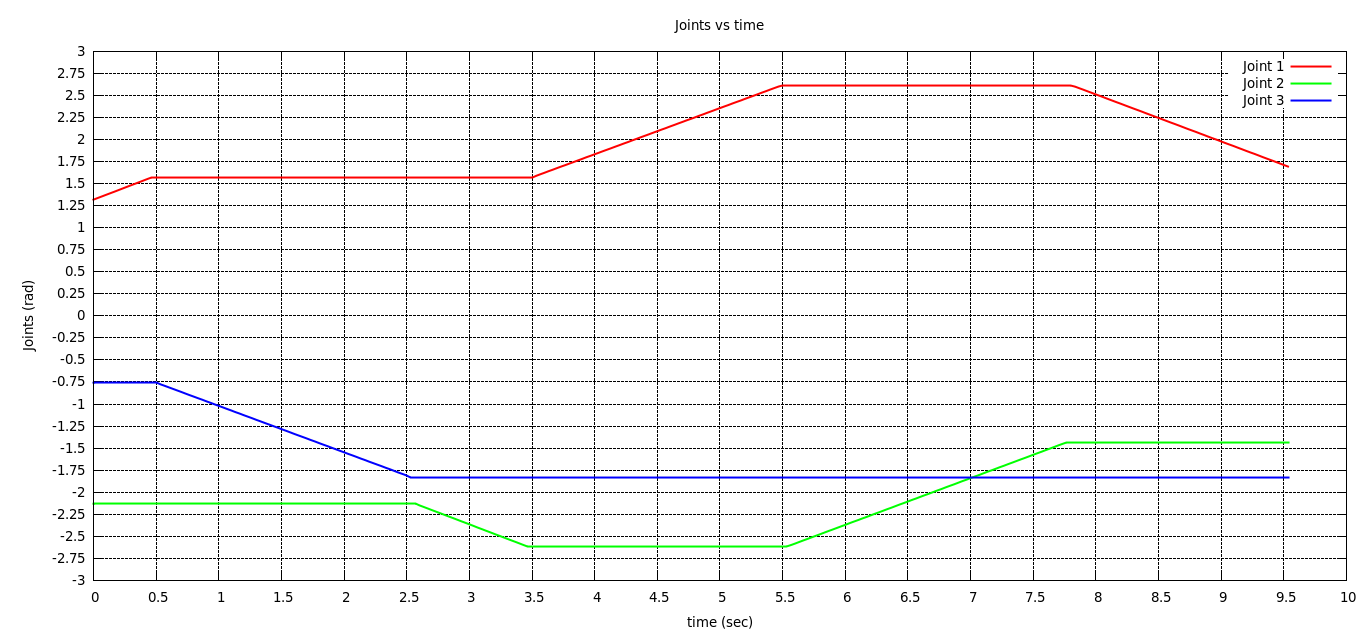
\includegraphics[angle = 0, scale = 0.3]{figures/Q3Joints.png} 
	\label{fig:Q3Joints}
	\caption{ Joints values for Question 3}
	\end{figure}

	\begin{figure}[H]
	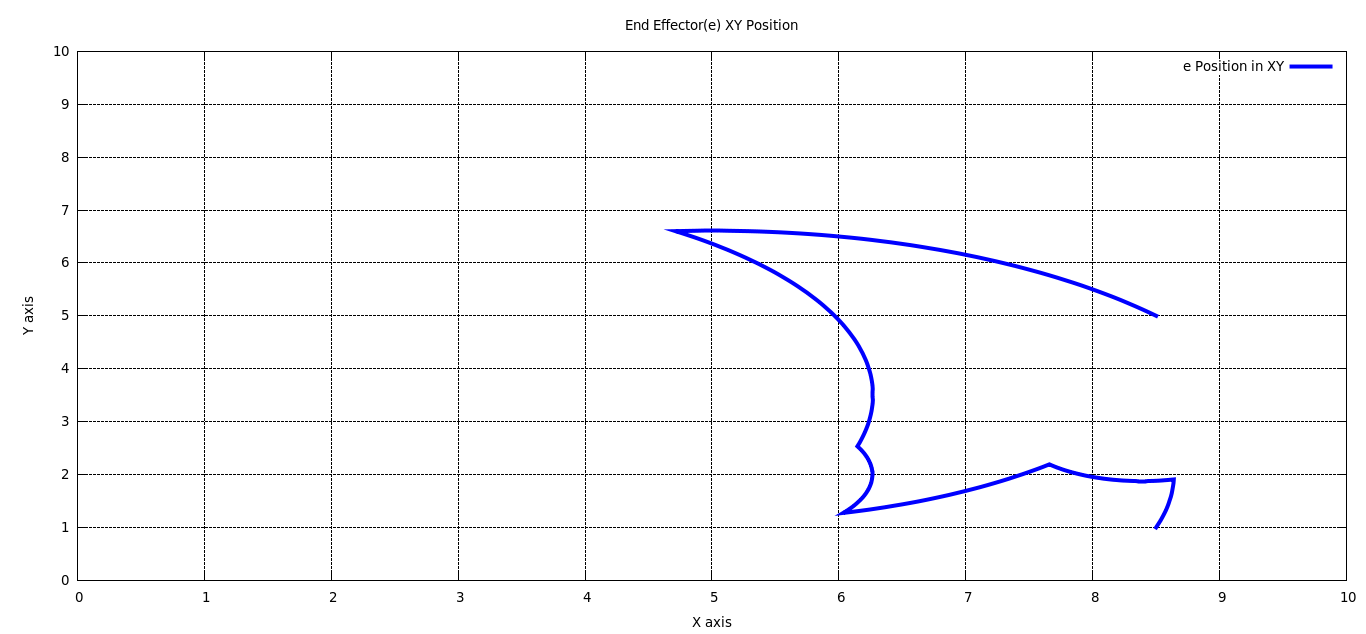
\includegraphics[angle = 0, scale = 0.3]{figures/Q3EEPos.png} 
	\label{fig:Q3EEPos}
	\caption{ End Effector Path for Question 3}
	\end{figure}
	
And here the robot plots while traversing the via points mentioned. Please take a look at the video attached.

	\begin{figure}[h]
			\centering
			  \subfigure[Position 0]{
			  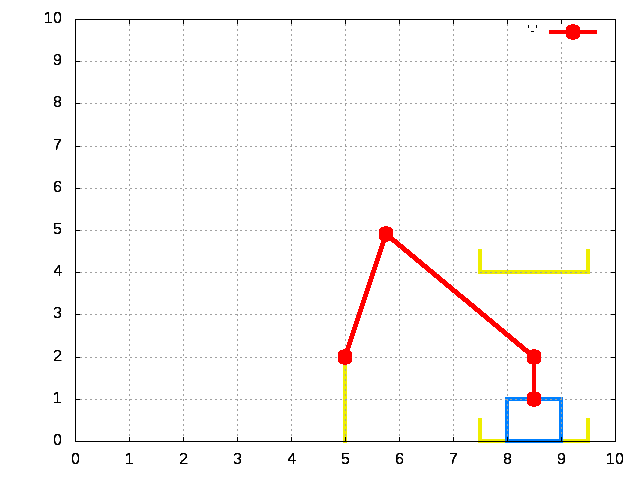
\includegraphics[scale=0.25]{figures/Q3Pos0.png} 
	          \label{fig:Q3Pos0}
              }
              \subfigure[Position 1]{
	          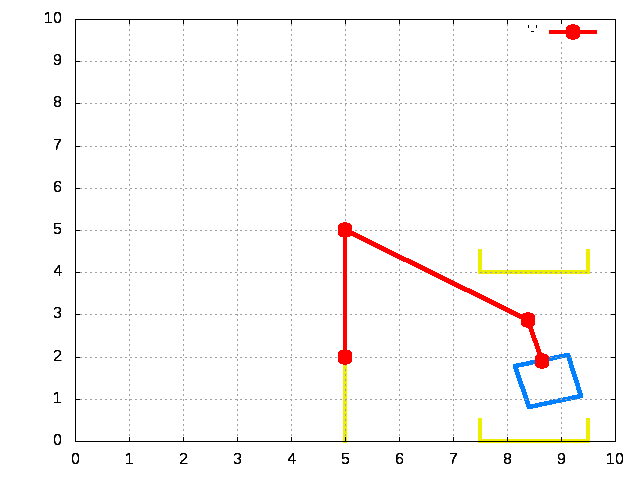
\includegraphics[scale=0.25]{figures/Q3Pos1.png} 	
	          \label{fig:Q3Pos1}
              }\\
			  \subfigure[Position 2]{
			  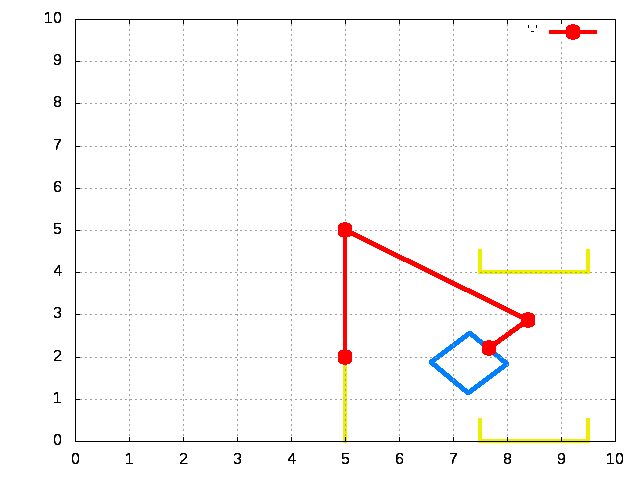
\includegraphics[scale=0.25]{figures/Q3Pos2.png} 
	          \label{fig:Q3Pos2}
              }
              \subfigure[Position 3]{
	          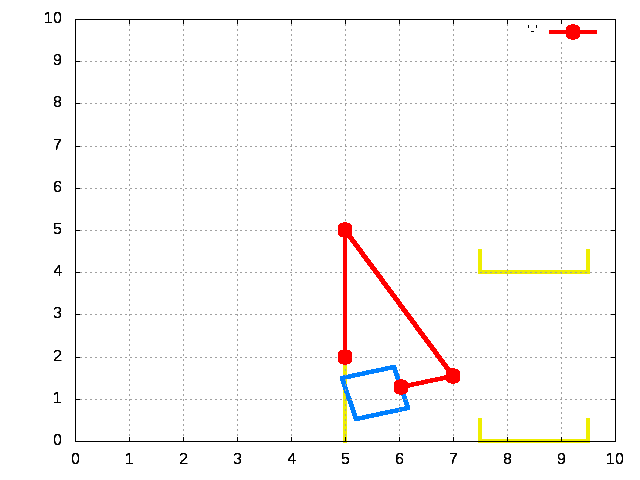
\includegraphics[scale=0.25]{figures/Q3Pos3.png} 	
	          \label{fig:Q3Pos3}
              }\\
              \subfigure[Position 4]{
			  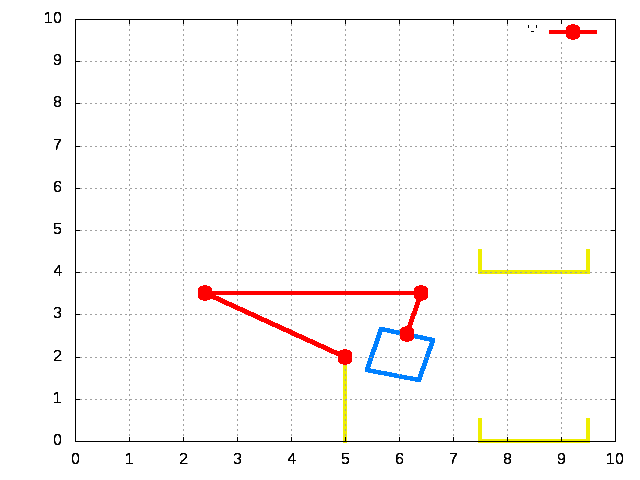
\includegraphics[scale=0.25]{figures/Q3Pos4.png} 
	          \label{fig:Q3Pos4}
              }
              \subfigure[Position 5]{
	          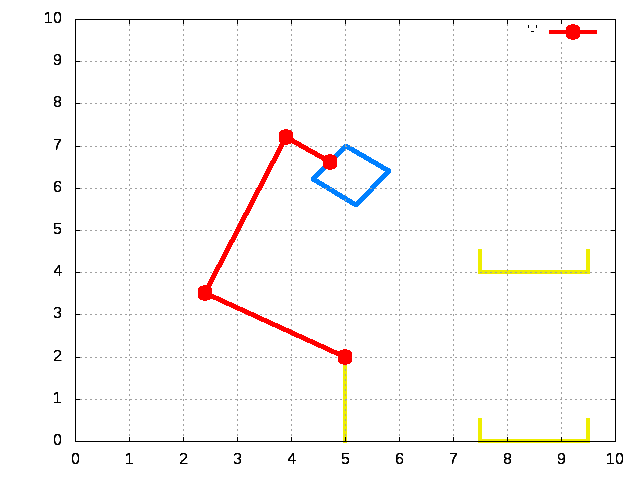
\includegraphics[scale=0.25]{figures/Q3Pos5.png} 	
	          \label{fig:Q3Pos5}
              }              
              \subfigure[Position 6]{
	          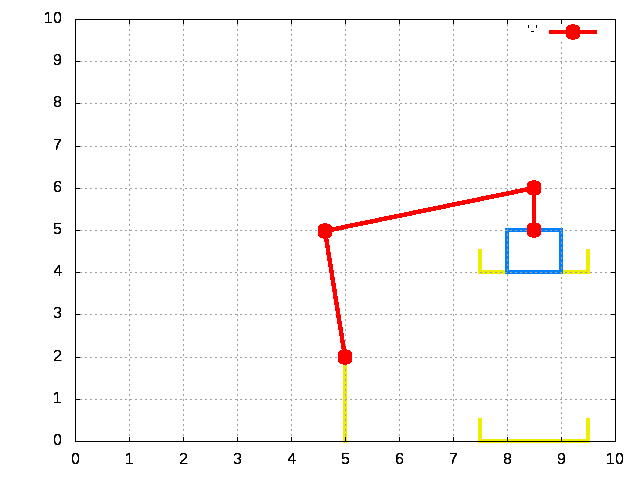
\includegraphics[scale=0.25]{figures/Q3Pos6.png} 	
	          \label{fig:Q3Pos6}
              } 
            \caption{ Robot poses for the trajectories plotted for question 3 }
            \label{fig:Q3}
	\end{figure}	

\end{document}